%------------------------------------------------
\section{Contributions}
%------------------------------------------------

% Intro à refaire 
%-----------------------------------------------------------------
\subsection{Relations aux triangulations de Delaunay}
%-----------------------------------------------------------------


L'enveloppe convexe est unique. Les algorithmes implantés fournissent les sommets dans l'ordre trigonométrique. Il est possible de reconstruire le polygône convexe et d'en déduire ses arêtes. Elles se décomposent en motif de droites discrètes. Un motif de droite discrète est inclue dans les segments de droites discrètes. La triangulation de Delaunay de ces motifs est connue. \cite{RoussillonL11}\\

\begin{figure}[H]
  \centering
  \includegraphics[width=0.5\linewidth]{fig/5-con/tri/con-motif-0.pdf}
  \caption{Triangulation de Delaunauy d'un motif de droite discrète}
\end{figure}

La triangulation de Delaunay dépend des convergents. Le dernier convergent différent de l'arête du segment de droite discrète est le sommet du triangle incident de la triangulation de Delaunay. À l'aide d'un calcul récursif, il est possible de construire l'intégralité de la triangulation de Delaunay.

\begin{figure}[H]
  \centering
  \includegraphics[width=0.5\linewidth]{fig/5-con/tri/con-conv-0.pdf}
  \caption{Calcul de concvergent et triangulation de Delaunauy}
\end{figure}

Comme les convergents sont calculés dans l'algorihtme de Har-Peled, il est probable de pouvoir construire l'$\alpha$-shape directement. 

%-----------------------------------------------------------------
\subsection{$\alpha$-shape, $\alpha \leq 0$ - Généralisation de Har-Peled}
%-----------------------------------------------------------------

%-----------------------------------------------------------------
\subsubsection{Construction de l'algorithme}

La méthode de calcul de l'$\alpha$-shape reproduire le schéma de départ du calcul de l’enveloppe convexe. Néanmoins, nous ajoutons une étape pour chaque convergent à l'intérieur du disque afin de contrôler la possibilité d'avoir construit une arête de l'$\alpha$-shape.

L'algorithme commence similairement par la recherche du point de départ. La même méthode sera utilisée pour trouver le point d'ordonnée minimale et d'abscisse maximale. Comme il appartient à l'enveloppe convexe, il appartient également à l'$\alpha$-shape.

À partir de ce point de départ, nous lancons une série de convergents pour étudier les arêtes $e$ potentiels. Les convergents se trouvent alternativement à l'intérieur de disque (convergent de degré impaire) et à l'extérieur où exactement sur le bord du disque (convergent de degré pair). À chaque convergent à l'intérieur (de couleur bleue foncé), on contrôle la possibilité d'avoir trouvé un sommet.

\begin{figure}[H]
  \centering
  \includegraphics[width=0.6\linewidth]{fig/5-con/nas/con-nas-0.pdf}
  \caption{Calcul des convergents}
\end{figure}

On note $b = p_{k-2} + (q_k - 1) * p_{k-1}$ et $c = p_k = p_{k-2} + q_k * p_{k-1}$. Pour savoir si c est un sommet, on utilise un prédicat qui compare la taille du rayon \textbf{$R_T$} du cercle circonscrit au triangle : $T(a, b, c)$ à la taille du rayon de notre disque généralisé : \textbf{$R_{\alpha}$} $= -1/\alpha$. Il faut distinguer deux cas de figures.\\

\begin{figure}[H]
  \centering
  \includegraphics[width=0.6\linewidth]{fig/5-con/nas/con-nas-1.pdf}
  \caption{Calcul du Prédicat}
\end{figure}

Si $\alpha = \alpha_{1}$ alors \textbf{$R_{\alpha_{1}} > R_T$} et le point b appartient au notre disque généralisé de rayon $-1/R_{\alpha_{1}}$ ( b appartient au complémentaire du disque de rayon $-1/R_{\alpha_{1}}$). On ne sait pas encore si le convergent c sera un sommet de l'$\alpha$-shape, mais on sait que b n'en sera pas un. Nous pouvons continuer le calcul des convergents.\\ 

Si $\alpha = \alpha_{2}$ alors \textbf{$R_{\alpha_{1}} < R_T$} et le point b n'appartient pas à notre disque généralisé de rayon $-1/R_{\alpha_{1}}$. L'$\alpha$-hull ne peut rejoindre c par a sans au moins passé par b. b et c appartiennent à notre $\alpha$-shape. Il faut maintenant vérifier si les points $b_i = p_{k-2} + i*p_{k-1} \forall i \in [0, q_k-2]$ appartiennent églament à l'$\alpha$-shape. \\

De part la construction des triangles, la taille des rayons de leur cercle circonscrit $R_{T_{i}}$ est croissante. Il suffit de tester le dernier et plus grand pour savoir si nous pouvons continuer notre algorithme et lancer les convergents suivants ou si nous devons déterminer quel sera le point $\alpha$-extrême par une recherche dichotomique. La recherche dichotomique permet de trouver en $log(q_k)$ le triangle adéquate $T_i = (a, b_{i}, b_{i+1}$ tel que $R_{T_i} > R_{\alpha}$ et $R_{T_{i-1}} \leq R_{\alpha}$.

\begin{figure}[H]
  \centering
  \includegraphics[trim = 1.2cm 1.2cm 1.2cm 0.6cm, clip,width=\linewidth]{fig/5-con/nas/con-nas-dicho.pdf}
  \caption{Taille croissante des rayons des cerlces circonscrits au triangle.}
\end{figure}

Le triangle renvoyé par la méthode dichotomique assure que l'ensemble des points $\left\{ b_{i},\ldots, b_{q_k}, c \right\}$ appartiennent à l'$\alpha$-shape. Nous continuons la méthode en repartant du sommet c.
 
\begin{figure}[H]
  \centering
  \includegraphics[trim = 1.2cm 1.2cm 1.2cm 0.6cm, clip,width=\linewidth]{fig/5-con/nas/con-nas-2.pdf}
  \caption{Nouveaux points et sommets de l'$\alpha$-shape.}
\end{figure}


%-----------------------------------------------------------------
\subsubsection{Résultats}

Les résultats présentés sont : 

\begin{figure}[H]
  \centering
  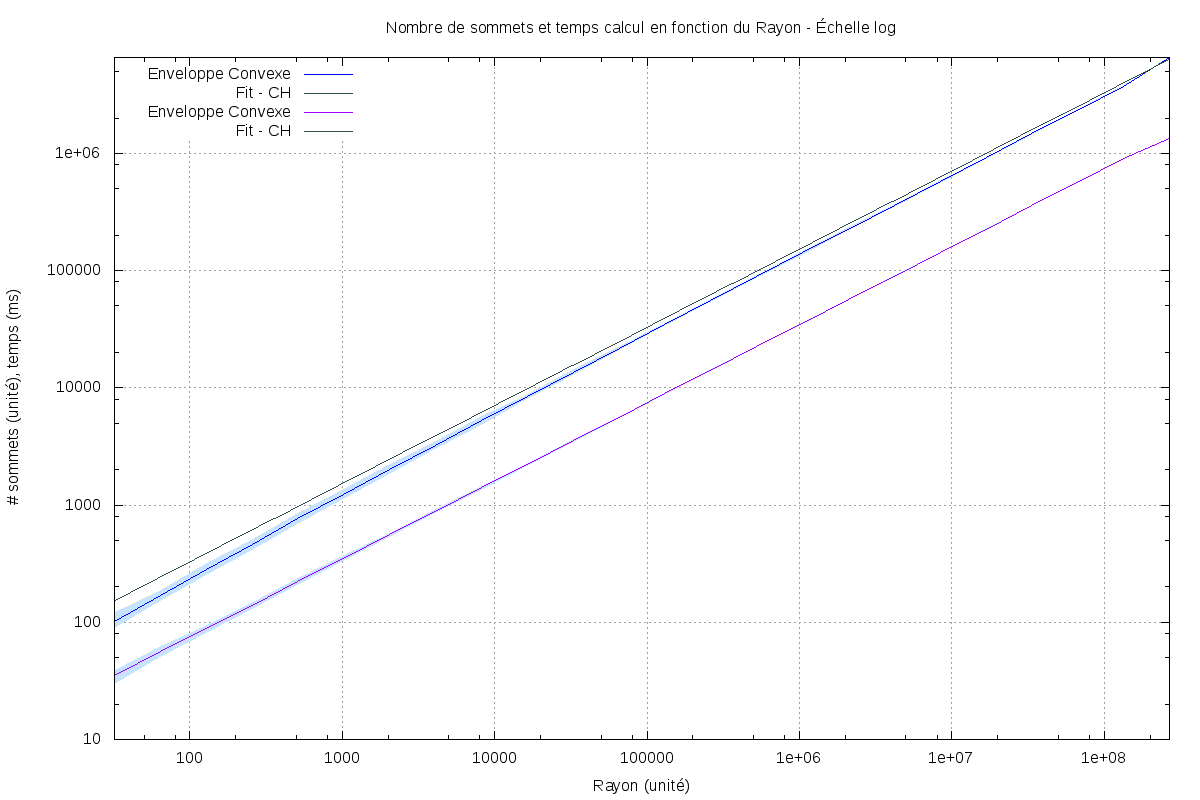
\includegraphics[width=\linewidth]{fig/4-exi/ch/exi-ch-sommet.png}
  \caption{Nombre de sommets de l'$\alpha$-shape en fonction de la taille des rayons. (Échelle log)}
\end{figure}


\begin{table}[H]
  \begin{tabular}{|p{0.09\linewidth}|p{0.13\linewidth}||p{0.23\linewidth}||p{0.23\linewidth}|p{0.23\linewidth}|}
    \hline
    \multicolumn{2}{|c||}{Rayon} & prédicat               & \multicolumn{2}{|c|}{$\alpha-shape$} \\  \hline 
    $R=2^k$  &                   & $-\alpha = R^{2}/1000$ & \multicolumn{2}{|c|}{Nombre de sommets} \\ \hline
    k        & R                 &                        & \# & $\# / R^{2/3}$ \\ 
    \hline
    5 & 32 & 1,024 & 179,02 & 17,761\\
    6 & 64 & 4,096 & 272,92 & 17,0575\\
    7 & 128 & 16,384 & 472,19 & 18,5913\\
    8 & 256 & 65,536 & 774,45 & 19,2088\\
    9 & 512 & 262,144 & 1,30E+03 & 20,3259\\
    10 & 1024 & 1,05E+03 & 2,14E+03 & 21,0878\\
    11 & 2048 & 4,19E+03 & 3,54E+03 & 21,9549\\
    12 & 4096 & 1,68E+04 & 5,68E+03 & 22,1878\\
    13 & 8192 & 6,71E+04 & 9,25E+03 & 22,7644\\
    14 & 16384 & 2,68E+05 & 1,49E+04 & 23,0413\\
    15 & 32768 & 1,07E+06 & 2,38E+04 & 23,2816\\
    16 & 65536 & 4,29E+06 & 3,84E+04 & 23,6175\\
    17 & 131072 & 1,72E+07 & 6,17E+04 & 23,9124\\
    18 & 262144 & 6,87E+07 & 9,89E+04 & 24,15\\
    19 & 524288 & 2,75E+08 & 1,59E+05 & 24,4137\\
    20 & 1048576 & 1,10E+09 & 2,54E+05 & 24,5914\\
    21 & 2097152 & 4,40E+09 & 4,06E+05 & 24,7603\\
    22 & 4194304 & 1,76E+10 & 6,49E+05 & 24,9402\\
    23 & 8388608 & 7,04E+10 & 1,04E+06 & 25,073\\
    24 & 16777216 & 2,81E+11 & 1,65E+06 & 25,2002\\
    25 & 33554432 & 1,13E+12 & 2,63E+06 & 25,3061\\
    26 &  &  &  & \\
    27 &  &  &  &  \\
    28 &  &  &  &  \\
    \hline
  \end{tabular} 
  \caption{Nombre de sommets de l'$\alpha$-shape}
\end{table}


%-----------------------------------------------------------------
\subsection{$\alpha$-shape, $\alpha \geq 0$}
%-----------------------------------------------------------------

%-----------------------------------------------------------------
\subsubsection{Construction de l'algorithme}


Notre version de l'algorithme s'appuie ici sur les sommets de l'enveloppe convexe. En effet, on va chercher à savoir quel sous-ensemble de point compose notre $\alpha$-shape.

%-----------------------------------------------------------------
\subsubsection{Résultats}

Les résultats présentés sont : 



